%%%%%%%%%%%%%%%%%%%%%%%%%%%%%%%%%%%%%%%%%%%%%%%%%%%%%%%%%%%%%%%%%%%
% Lostify — University Presentation (Beamer)
% Compile: pdflatex FINAL_PRESENTATION.tex (twice if needed)
% Place logo.jpg in Bilder/ folder next to this file
%%%%%%%%%%%%%%%%%%%%%%%%%%%%%%%%%%%%%%%%%%%%%%%%%%%%%%%%%%%%%%%%%%%
\documentclass[11pt,aspectratio=169]{beamer}

\usetheme{Madrid}
\usecolortheme{default}
\setbeamertemplate{navigation symbols}{}
\setbeamertemplate{footline}[frame number]

\usepackage[T1]{fontenc}
\usepackage[english]{babel}
\usepackage{graphicx}
\usepackage{booktabs}
\usepackage{tikz}
\usetikzlibrary{shapes.geometric, arrows.meta, positioning}
\usepackage{hyperref}

\graphicspath{{Bilder/}}

\title{Lostify}
\subtitle{Lost \& Found Microservices Platform}
\author{Zain Afzal \and Babar Ali \and Muhammad Hamza Azeem}
\institute{Team 04 \quad|\quad Serverless Cloud Application Automation\\Prof.\ Sashko Ristov}
\date{July 1, 2026}

% Compact lists
\setbeamertemplate{itemize items}[circle]
\setlength{\leftmargini}{1.2em}

\begin{document}

% ── Title ──────────────────────────────────────────────────────
\begin{frame}
  \titlepage
  \vspace{-0.8cm}
  \centering
  \footnotesize
  \href{https://github.com/Babarali2k21/Lostify}{github.com/Babarali2k21/Lostify}
  \quad|\quad
  \href{http://44.220.148.111:3001}{Live demo :3001}
\end{frame}

% ── Outline ────────────────────────────────────────────────────
\begin{frame}{Outline}
  \tableofcontents
\end{frame}

% ==============================================================
\section{Introduction}
% ==============================================================

\begin{frame}{The Problem}
  \begin{itemize}
    \item People lose items daily in universities, libraries, offices, public transport.
    \item Recovery is often \textbf{manual}: phone calls, physical desks, chat groups.
    \item Hard to track: Was there a match? Was the owner notified? Was handover completed?
  \end{itemize}
  \vspace{0.6cm}
  \begin{block}{Our goal}
    A digital lost-and-found platform with automatic matching, notifications and a controlled claim workflow.
  \end{block}
\end{frame}

\begin{frame}{What Lostify Demonstrates}
  \begin{columns}[T]
    \column{0.48\textwidth}
    \textbf{Architecture}
    \begin{itemize}
      \item Microservice decomposition
      \item Database per service
      \item API composition
    \end{itemize}
    \column{0.48\textwidth}
    \textbf{Distributed systems}
    \begin{itemize}
      \item Saga pattern + compensation
      \item Event-driven notifications
      \item Redis pub/sub
    \end{itemize}
  \end{columns}
  \vspace{0.4cm}
  \begin{columns}[T]
    \column{0.48\textwidth}
    \textbf{Cloud \& automation}
    \begin{itemize}
      \item Docker on AWS EC2
      \item AWS Step Functions
      \item GitHub Actions CI/CD
    \end{itemize}
    \column{0.48\textwidth}
    \textbf{Evaluation}
    \begin{itemize}
      \item 31 automated tests
      \item Fault tolerance
      \item Latency + lead time
    \end{itemize}
  \end{columns}
\end{frame}

% ==============================================================
\section{Architecture}
% ==============================================================

\begin{frame}{Three Business Microservices}
  \begin{block}{Design decision (course feedback)}
    \textbf{No User microservice.} JWT register/login lives inside Item Service as application-level auth.
  \end{block}
  \vspace{0.3cm}
  \small
  \begin{tabular}{@{}llp{5.5cm}@{}}
    \toprule
    \textbf{Service} & \textbf{Port} & \textbf{Responsibility} \\
    \midrule
    Item Service         & 8001 & Auth, items, matching, item states \\
    Claim/Recovery Svc   & 8002 & Claims, Saga, compensation, Step Functions \\
    Notification Service & 8003 & Redis consumer, deduplication, notification log \\
    \bottomrule
  \end{tabular}
\end{frame}

\begin{frame}{System Architecture}
  \centering
  \resizebox{0.95\textwidth}{!}{%
  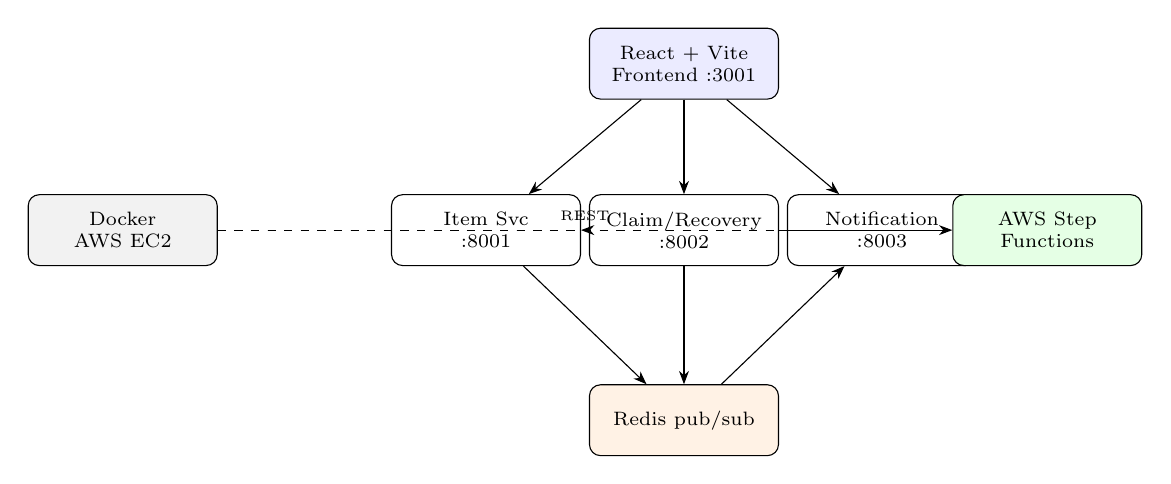
\begin{tikzpicture}[
    box/.style={draw, rounded corners, align=center, font=\scriptsize,
                minimum width=2.4cm, minimum height=0.9cm, inner sep=3pt},
    >=Stealth, node distance=1.1cm and 1.5cm
  ]
    \node[box, fill=blue!8] (web) {React + Vite\\Frontend :3001};
    \node[box, below left=1.2cm and 0.1cm of web] (item) {Item Svc\\:8001};
    \node[box, below=1.2cm of web] (claim) {Claim/Recovery\\:8002};
    \node[box, below right=1.2cm and 0.1cm of web] (notif) {Notification\\:8003};
    \node[box, below=1.5cm of claim, fill=orange!10] (redis) {Redis pub/sub};
    \node[box, right=2.2cm of claim, fill=green!10] (sf) {AWS Step\\Functions};
    \node[box, left=2.2cm of item, fill=gray!10] (ec2) {Docker\\AWS EC2};

    \draw[->] (web) -- (item);
    \draw[->] (web) -- (claim);
    \draw[->] (web) -- (notif);
    \draw[->] (item) -- (redis);
    \draw[->] (claim) -- (redis);
    \draw[->] (redis) -- (notif);
    \draw[->] (claim) -- node[above,font=\tiny]{REST} (item);
    \draw[->] (claim) -- (sf);
    \draw[dashed] (ec2) -- (item);
    \draw[dashed] (ec2) -- (claim);
    \draw[dashed] (ec2) -- (notif);
  \end{tikzpicture}
  }
  \vspace{0.2cm}
  \footnotesize Each service owns its own SQLite database. Frontend nginx proxies \texttt{/api/item/*}, \texttt{/api/claim/*}, \texttt{/api/notif/*}.
\end{frame}

\begin{frame}{End-to-End User Flow}
  \begin{enumerate}
    \item Register \& login \hfill $\rightarrow$ Item Service
    \item Create lost + found reports \hfill $\rightarrow$ Item Service
    \item Keyword matching finds pair \hfill $\rightarrow$ status \texttt{MATCHED}
    \item \texttt{MatchFound} event \hfill $\rightarrow$ Notification Service
    \item User submits claim \hfill $\rightarrow$ Claim/Recovery Service
    \item Saga reserves item \hfill $\rightarrow$ \texttt{RESERVED}
    \item Finder approves or rejects
    \item Approve: \texttt{RECOVERED} \quad|\quad Reject: compensation $\rightarrow$ \texttt{MATCHED}
  \end{enumerate}
  \vspace{0.3cm}
  \centering\small\texttt{ItemCreated → ItemCreated → MatchFound → ClaimCreated → ClaimApproved → ItemRecovered}
\end{frame}

% ==============================================================
\section{Saga \& Events}
% ==============================================================

\begin{frame}{Item \& Claim State Machines}
  \begin{columns}[T]
    \column{0.48\textwidth}
    \textbf{Item lifecycle}
    \vspace{0.2cm}
    \centering\small
    \texttt{OPEN} $\rightarrow$ \texttt{MATCHED} $\rightarrow$ \texttt{RESERVED} $\rightarrow$ \texttt{RECOVERED}\\
    \vspace{0.2cm}
    Reject: \texttt{RESERVED} $\rightarrow$ \texttt{MATCHED}
    \column{0.48\textwidth}
    \textbf{Claim lifecycle}
    \vspace{0.2cm}
    \centering\small
    \texttt{PENDING} $\rightarrow$ \texttt{APPROVED}\\
    \texttt{PENDING} $\rightarrow$ \texttt{REJECTED}
  \end{columns}
  \vspace{0.5cm}
  \begin{block}{Saga orchestration}
    Claim/Recovery Service runs \texttt{ClaimRecoverySaga} locally and calls Item Service REST:
    \texttt{/items/\{id\}/reserve}, \texttt{/release}, \texttt{/recover}
  \end{block}
\end{frame}

\begin{frame}{Saga: Happy Path vs Compensation}
  \centering
  \resizebox{0.92\textwidth}{!}{%
  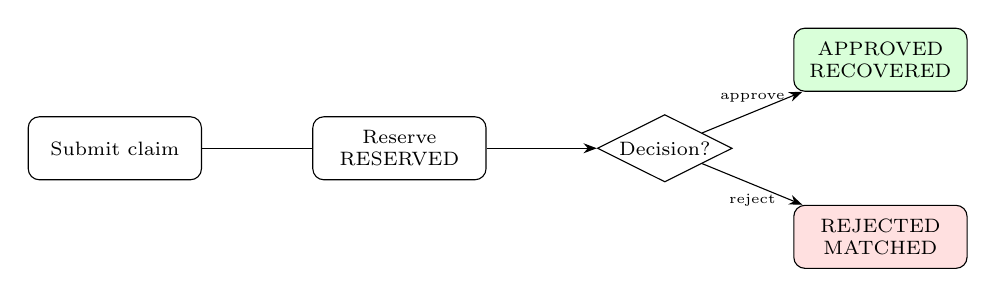
\begin{tikzpicture}[
    state/.style={draw, rounded corners, align=center, font=\scriptsize,
                  minimum width=2.2cm, minimum height=0.8cm},
    decision/.style={draw, diamond, aspect=2, align=center, font=\scriptsize, inner sep=1pt},
    >=Stealth, node distance=0.9cm and 1.4cm
  ]
    \node[state] (s) {Submit claim};
    \node[state, right=of s] (r) {Reserve\\RESERVED};
    \node[decision, right=of r] (d) {Decision?};
    \node[state, above right=0.5cm and 1.2cm of d, fill=green!15] (ok) {APPROVED\\RECOVERED};
    \node[state, below right=0.5cm and 1.2cm of d, fill=red!12] (no) {REJECTED\\MATCHED};
    \draw[->] (s) -- (r) -- (d);
    \draw[->] (d) -- node[above,font=\tiny]{approve} (ok);
    \draw[->] (d) -- node[below,font=\tiny]{reject} (no);
  \end{tikzpicture}
  }
  \vspace{0.4cm}
  \small Compensation = forward update (release item), \textbf{not} a database rollback.
\end{frame}

\begin{frame}{Event-Driven Communication}
  \textbf{Redis pub/sub} channel: \texttt{lostify:events}
  \vspace{0.3cm}
  \begin{columns}[T]
    \column{0.55\textwidth}
    \textbf{Event types}
    \begin{itemize}
      \item \texttt{ItemCreated}, \texttt{MatchFound}
      \item \texttt{ClaimCreated}, \texttt{ClaimApproved}
      \item \texttt{ClaimRejected}, \texttt{ItemRecovered}
    \end{itemize}
    \column{0.42\textwidth}
    \textbf{Deduplication}
    \begin{itemize}
      \item Every event has \texttt{eventId}
      \item Notification Service stores processed IDs
      \item Duplicates ignored
    \end{itemize}
  \end{columns}
  \vspace{0.3cm}
  \begin{block}{Why events?}
    Item and Claim services do not call Notification Service directly --- loose coupling, independent scaling.
  \end{block}
\end{frame}

% ==============================================================
\section{Technology \& AWS}
% ==============================================================

\begin{frame}{Technology Stack}
  \small
  \begin{tabular}{@{}ll@{}}
    \toprule
    \textbf{Component} & \textbf{Choice} \\
    \midrule
    Frontend      & React 18 + Vite + nginx (:3001) \\
    Backend       & Python 3.12 + FastAPI (3 services) \\
    Databases     & SQLite per service (RDS upgrade path) \\
    Event bus     & Redis 7 pub/sub \\
    Containers    & Docker + Docker Compose \\
    Cloud host    & AWS EC2 Ubuntu 24.04 (\texttt{t3.small}) \\
    Workflow      & AWS Step Functions + 5 Lambda functions \\
    CI/CD         & GitHub Actions \\
    Region        & \texttt{eu-central-1} \\
    \bottomrule
  \end{tabular}
\end{frame}

\begin{frame}{AWS Deployment}
  \begin{itemize}
    \item Full stack runs on \textbf{one EC2 instance} via \texttt{docker-compose.prod.yml}
    \item Redis \textbf{not exposed} publicly (internal only)
    \item Security group: SSH (22), frontend (3001), services (8001--8003)
    \item Automated deploy: GitHub Actions rsync $\rightarrow$ EC2 $\rightarrow$ rebuild
  \end{itemize}
  \vspace{0.4cm}
  \begin{columns}[T]
    \column{0.48\textwidth}
    \textbf{Live demo}
    \begin{itemize}
      \item \url{http://44.220.148.111:3001}
      \item Health via proxy:
      \texttt{/api/item/health}
    \end{itemize}
    \column{0.48\textwidth}
    \textbf{Step Functions}
    \begin{itemize}
      \item State machine: \texttt{ClaimRecoverySaga}
      \item Same steps as local Saga
      \item Frontend shows AWS sync status
    \end{itemize}
  \end{columns}
\end{frame}

\begin{frame}{AWS Step Functions}
  \centering\small
  \texttt{CreateClaim → ReserveItem → NotifyClaimCreated → Choice}
  \vspace{0.2cm}
  \begin{columns}[T]
    \column{0.48\textwidth}
    \textbf{APPROVED path}
    \begin{itemize}
      \item RecoverItem
      \item NotifyClaimApproved
      \item NotifyItemRecovered
      \item $\rightarrow$ SagaSucceeded
    \end{itemize}
    \column{0.48\textwidth}
    \textbf{REJECTED path}
    \begin{itemize}
      \item ReleaseItem (compensation)
      \item NotifyClaimRejected
      \item $\rightarrow$ SagaCompensated
    \end{itemize}
  \end{columns}
  \vspace{0.3cm}
  \footnotesize Local = choreography (Saga in code). AWS = orchestration (visual graph for presentation).
\end{frame}

\begin{frame}{CI/CD Pipeline}
  \centering
  \resizebox{0.88\textwidth}{!}{%
  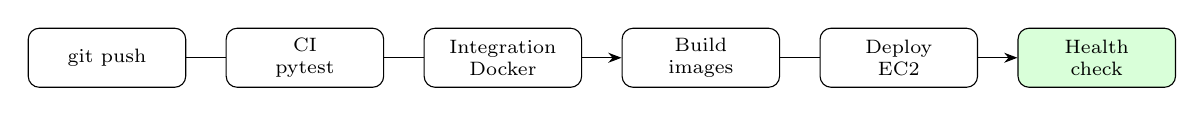
\begin{tikzpicture}[
    box/.style={draw, rounded corners, align=center, font=\scriptsize,
                minimum width=2.0cm, minimum height=0.75cm},
    >=Stealth, node distance=0.5cm
  ]
    \node[box] (git) {git push};
    \node[box, right=of git] (ci) {CI\\pytest};
    \node[box, right=of ci] (int) {Integration\\Docker};
    \node[box, right=of int] (build) {Build\\images};
    \node[box, right=of build] (dep) {Deploy\\EC2};
    \node[box, right=of dep, fill=green!15] (ok) {Health\\check};
    \draw[->] (git) -- (ci) -- (int) -- (build);
    \draw[->] (build) -- (dep) -- (ok);
  \end{tikzpicture}
  }
  \vspace{0.5cm}
  \begin{itemize}
    \item Workflows: \texttt{ci.yml} + \texttt{deploy.yml}
    \item Deploy reports to GitHub \texttt{production} environment
    \item \textbf{Lead time: 3--5 minutes} from commit to live EC2
  \end{itemize}
\end{frame}

% ==============================================================
\section{Evaluation}
% ==============================================================

\begin{frame}{Evaluation Overview}
  \textbf{31 automated tests}
  \vspace{0.2cm}
  \small
  \begin{tabular}{@{}lrl@{}}
    \toprule
    \textbf{Category} & \textbf{Count} & \textbf{Examples} \\
    \midrule
    Unit (events, saga, dedup, Step Fn) & 22 & Saga approve/reject, event serialization \\
    Integration (E2E)                   &  2 & Full demo flow, reject compensation \\
    Fault tolerance                     &  5 & Duplicates, auth errors, invalid states \\
    Event latency                       &  2 & MatchFound, ClaimCreated $<$ 5 s \\
    \bottomrule
  \end{tabular}
  \vspace{0.4cm}
  \texttt{./scripts/run-all-tests.sh} \quad|\quad \texttt{./scripts/evaluation-report.sh}
\end{frame}

\begin{frame}{Key Evaluation Results}
  \small
  \begin{tabular}{@{}ll@{}}
    \toprule
    \textbf{Metric} & \textbf{Result} \\
    \midrule
    All automated tests        & Pass (31/31 when Docker healthy) \\
    MatchFound latency (local) & 50--500 ms typical \\
    Duplicate event handling   & PASS (deduplication verified) \\
    Claim rejection compensation & Item returns to \texttt{MATCHED} \\
    CI + deploy lead time      & $\sim$3--5 min \\
    EC2 health check           & 3/3 services OK \\
    \bottomrule
  \end{tabular}
  \vspace{0.4cm}
  \begin{block}{Fault tolerance verified}
    Duplicate events ignored \quad|\quad Wrong user blocked (403) \quad|\quad Invalid transitions rejected (400)
  \end{block}
\end{frame}

\begin{frame}{Live Demo Plan}
  \textbf{During presentation — show:}
  \begin{enumerate}
    \item Open \url{http://44.220.148.111:3001} — register two users
    \item Create lost item (Alice) + found item (Bob) $\rightarrow$ match notification
    \item Submit claim $\rightarrow$ saga panel shows \texttt{AWAITING\_DECISION}
    \item Approve $\rightarrow$ \texttt{RECOVERED} + events in panel
    \item (Optional) Reject path $\rightarrow$ compensation to \texttt{MATCHED}
    \item AWS Console: Step Functions graph — green execution
    \item GitHub: Actions tab — green CI + Deploy
  \end{enumerate}
  \vspace{0.2cm}
  \footnotesize Backup: \texttt{./scripts/demo.sh} and \texttt{./scripts/demo\_reject.sh}
\end{frame}

% ==============================================================
\section{Wrap-up}
% ==============================================================

\begin{frame}{Limitations \& Future Work}
  \begin{columns}[T]
    \column{0.48\textwidth}
    \textbf{Current limitations}
    \begin{itemize}
      \item Keyword matching (simple)
      \item SQLite (not RDS yet)
      \item No email (SES future)
      \item No claim cancellation
      \item Mock Lambda handlers
    \end{itemize}
    \column{0.48\textwidth}
    \textbf{Future work}
    \begin{itemize}
      \item PostgreSQL on RDS
      \item Better matching + images (S3)
      \item Email via SES
      \item Live Lambda $\rightarrow$ EC2 APIs
      \item Kubernetes / ECS scaling
    \end{itemize}
  \end{columns}
\end{frame}

\begin{frame}{Team Contributions}
  \small
  \begin{tabular}{@{}lp{9.5cm}@{}}
    \toprule
    \textbf{Member} & \textbf{Contribution} \\
    \midrule
    Zain Afzal &
    Notification Service, Redis events, deduplication, integration tests \\[0.3em]
    Babar Ali &
    Claim/Recovery Service, Saga, Step Functions, EC2 deploy, GitHub Actions \\[0.3em]
    Muhammad Hamza Azeem &
    Item Service, matching, item states, auth merge, workflow tests \\
    \bottomrule
  \end{tabular}
\end{frame}

\begin{frame}{Conclusion}
  \begin{itemize}
    \item Lostify = \textbf{3 microservices} + event-driven notifications + Saga with compensation
    \item Auth correctly embedded in Item Service (not a 4th microservice)
    \item Deployed on \textbf{AWS EC2}, visualized with \textbf{Step Functions}, delivered via \textbf{GitHub Actions}
    \item \textbf{31 tests} + live demo prove functional, fault-tolerant and automated delivery
  \end{itemize}
  \vspace{0.6cm}
  \centering
  \Large\textbf{Questions?}
  \vspace{0.3cm}

  \footnotesize
  \href{https://github.com/Babarali2k21/Lostify}{github.com/Babarali2k21/Lostify}
  \quad|\quad
  \href{http://44.220.148.111:3001}{44.220.148.111:3001}
\end{frame}

\end{document}
